\documentclass[12pt]{article}

\usepackage[margin=1in]{geometry}
\usepackage{tabularx}
\usepackage{booktabs}
\usepackage{amsmath}
\usepackage{times}
\usepackage[utf8]{inputenc}
\usepackage{tikz}
\usepackage[compat=1.1.0]{tikz-feynman}

\newcolumntype{Y}{>{\centering\arraybackslash}X}
\newcolumntype{B}{>{\hsize=.15\hsize}Y}
\newcolumntype{M}{>{\hsize=.25\hsize}Y}
\newcolumntype{S}{>{\hsize=.05\hsize}Y}

\begin{document}
    
%% Change \toperule to \hline\hline if you prefer the two separate lines in the table

\begin{table}\centering
    \caption{Experimental and theoretical systematic uncertainties for 2016 data.}
    \begin{tabularx}{.7\textwidth}{>{\hsize=.8\hsize}X>{\hsize=.2\hsize}Y}\toprule
        \multicolumn{2}{c}{\textbf{Summary of relative systematic uncertainties}} \\ \toprule
        \multicolumn{2}{c}{Common experimental uncertainties} \\ \hline
        Luminosity & 2.6 \% \\
        Lepton identification / reconstruction efficiencies & 2.5 -- 9 \% \\
        Lepton energy scale & 0.1 -- 12.7 \% \\
        Lepton energy resolution & 0.01 -- 4.7 \% \\ \toprule
        
        \multicolumn{2}{c}{Common theory-related uncertainties} \\ \hline
        Higgs branching fraction & 2 \% \\
        QCD scale & 0.4 -- 4.2 \% \\
        PDF scale & 1.6 -- 3.4 \% \\ \toprule
        
        \multicolumn{2}{c}{Background-related uncertainties} \\ \hline
        Reducible background (Z+X) & 53 -- 79 \% \\
        $q\bar{q} \rightarrow 4l$ electroweak correction & 0.1 \% \\
        $gg \rightarrow 4l$ kfactor & 10.0 \% \\ \toprule
        
        \multicolumn{2}{c}{Signal-related uncertainties} \\ \hline
        Interference & 2.0 \% \\
        QCD scale & 0.4 -- 4.2 \% \\
        PDF scale & 1.6 -- 3.4 \% \\
        Branching ratio & 10 -- 20 \% \\ \toprule
        
    \end{tabularx}
\end{table}

\begin{figure}\centering
    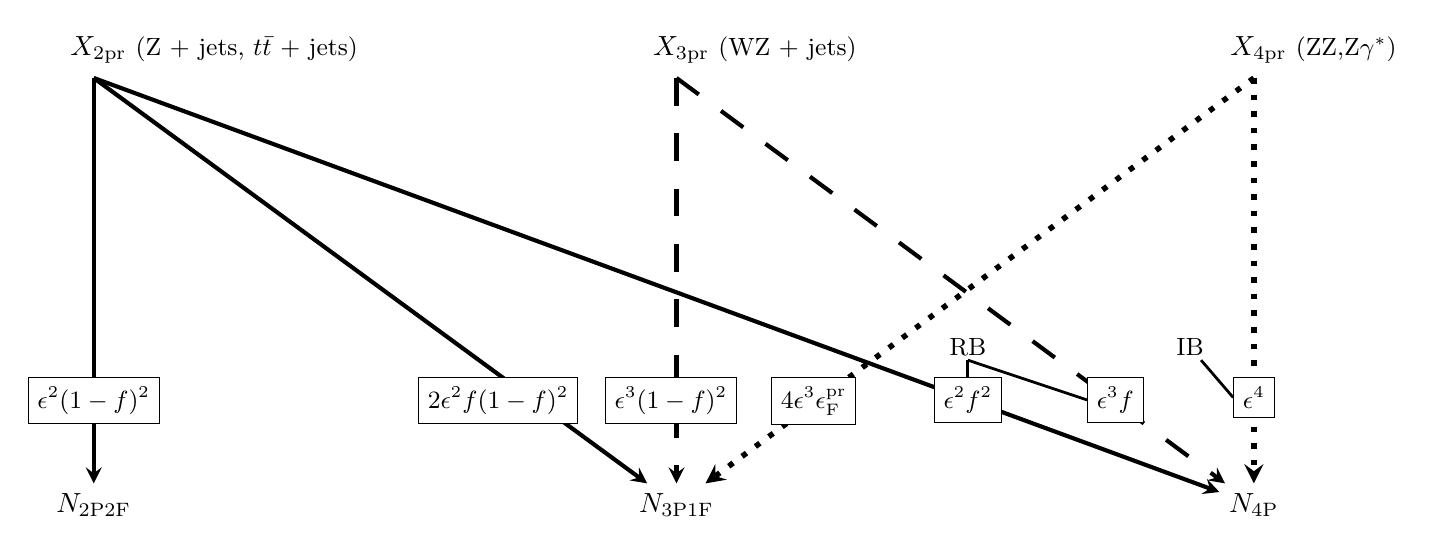
\begin{tikzpicture}
        % top nodes
        \node[yshift=5pt] (X2pr) {$X_\text{2pr}$ {\small (Z + jets, $t\bar{t}$ + jets)}};
        \node[right=3.5cm of X2pr] (X3pr) {$X_\text{3pr}$ {\small(WZ + jets)}};
        \node[right=4.5cm of X3pr] (X4pr) {$X_\text{4pr}$ {\small(ZZ,Z$\gamma^*$)}};
        
        % bottom nodes
        \node[below=5.5cm of X2pr.west, xshift=12pt] (N2P2F) {$N_\text{2P2F}$};
        \node[below=5.5cm of X3pr.west, xshift=12pt] (N3P1F) {$N_\text{3P1F}$};
        \node[below=5.5cm of X4pr.west, xshift=12pt] (N4P) {$N_\text{4P}$};
        
        % solid lines
        \draw[-stealth, line width=1.5pt] ([yshift=-10pt,xshift=12pt]X2pr.west) -- (N2P2F);
        \draw[-stealth, line width=1.5pt] ([yshift=-10pt,xshift=12pt]X2pr.west) -- (N3P1F);
        \draw[-stealth, line width=1.5pt] ([yshift=-10pt,xshift=12pt]X2pr.west) -- (N4P);

        % dashed lines
        \draw[-stealth, dash pattern=on 10pt off 10pt, line width=1.5pt] ([yshift=-10pt,xshift=12pt]X3pr.west) -- (N3P1F);
        \draw[-stealth, dash pattern=on 10pt off 10pt, line width=1.5pt] ([yshift=-10pt,xshift=12pt]X3pr.west) -- (N4P);
        
        % dotted lines
        \draw[-stealth, loosely dotted, line width=2pt] ([yshift=-10pt,xshift=12pt]X4pr.west) -- (N3P1F);
        \draw[-stealth, loosely dotted, line width=2pt] ([yshift=-10pt,xshift=12pt]X4pr.west) -- (N4P);
        
        % equation nodes
        \node[draw, fill=white, below=4.15 of X2pr.west, xshift=12pt] (eq1) {\small $\epsilon^2(1-f)^2$};
        \node[draw, fill=white, below left=4.15 and 1.25cm of X3pr.west, xshift=12pt] (eq2) {\small $2\epsilon^2f(1-f)^2$};
        \node[draw, fill=white, below=4.15 of X3pr.west, xshift=10pt] (eq3) {\small $\epsilon^3(1-f)^2$};
        \node[draw, fill=white, below right=4.15 and 1.2cm of X3pr.west, xshift=12pt] (eq4) {\small $4\epsilon^3\epsilon_\text{F}^\text{pr}$};
        \node[draw, fill=white, below left=4.15 and 3.2cm of X4pr.west, xshift=12pt] (eq5) {\small $\epsilon^2f^2$};
        \node[draw, fill=white, below left=4.15 and 1.4cm of X4pr.west, xshift=12pt] (eq6) {\small $\epsilon^3f$};
        \node[draw, fill=white, below=4.15 of X4pr.west, xshift=12pt] (eq7) {\small $\epsilon^4$};

        % RB and IB nodes
        \node[fill=white, above=.25cm of eq5, yshift=-3pt] (RB) {\small RB};
        \node[fill=white, above left=.25cm and 0.25cm of eq7, yshift=-3pt] (IB) {\small IB};

        \draw[line width=1pt] ([yshift=2pt]RB.south) -- (eq5.north);
        \draw[line width=1pt] ([yshift=2pt]RB.south) -- (eq6.west);
        \draw[line width=1pt] ([yshift=2pt,xshift=4pt]IB.south) -- (eq7.west);
        
        % \draw[line width=1.5pt, -stealth] (e21f2) -- (N2P2F);
        
        % \diagram* {
            % (X2pr) -- (e21f2),
        %     (ZZ) -- [boson, edge label=$Z$] (Z1),
        %     (ZZ) -- [boson, edge label=$Z$] (Z2),
        %     (Z1) -- [boson, edge label=$Z_D$] (ZD),
        %     (ZDl2) -- [fermion] (ZD) -- [fermion] (ZDl1);
        %     (Z2l2) -- [fermion] (Z2) -- [fermion] (Z2l1);
        % };
    \end{tikzpicture}
    \caption{Contributions of per-event weights (boxed values) of various $n$-prompt-lepton processes ($X_\text{npr}$, in parentheses) to the total numbers of events in the observed control region ($N_\text{2P2F}$,$N_\text{4P}$). The labels ``IB'' and ``RB'' indicate those contributions which comprise the irreducible and reducible backgrounds, respectively.}
\end{figure}

\begin{figure}[ht]
    \centering
    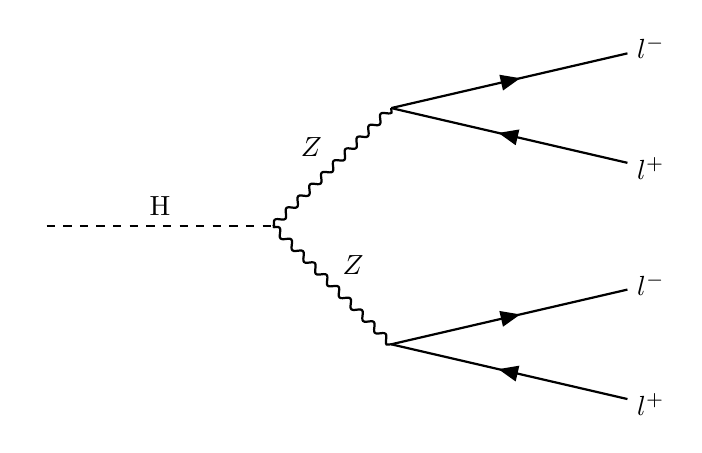
\begin{tikzpicture}

    \begin{feynman}[large]
        \vertex (h) {}; % h at beginning 
        \vertex [right=3cm of h] (s); % s -> ZDZD vertex
        \vertex [above right = 1.5cm and 1.5cm of s] (Z1); % top ZD
        \vertex [below right = 1.5cm and 1.5cm of s] (Z2); % bottom ZD
        \vertex [above right = 0.5cm and 3cm of Z2] (Z2l1) {$l^-$}; % top l of top Z
        \vertex [below right = 0.5cm and 3cm of Z2] (Z2l2) {$l^+$}; % bottom l of top Z
        \vertex [above right = 0.5cm and 3cm of Z1] (Z1l1) {$l^-$}; % top l of bottom Z
        \vertex [below right = 0.5cm and 3cm of Z1] (Z1l2) {$l^+$}; % bottom l of bottom Z
        
        \diagram* {
            (h) -- [scalar, edge label=H] (s),
            % (kappa) -- [scalar, edge label=$s$, below] (s),
            (s) -- [boson, edge label=$Z$] (Z1),
            (s) -- [boson, edge label=$Z$] (Z2),
            (Z1l2) -- [fermion] (Z1) -- [fermion] (Z1l1);
            (Z2l2) -- [fermion] (Z2) -- [fermion] (Z2l1);
        };
    \end{feynman}
    \end{tikzpicture}
    \caption{Feynman diagram showing how different physics processes can have the same initial and final states.}
\end{figure}

\end{document}